\documentclass[12pt]{article}
\usepackage[utf8]{inputenc}
\usepackage{graphicx}
\graphicspath{{images/}}
\usepackage{verbatim}
\usepackage{hyperref}

% Title Packages
\usepackage{titling}

% Timeline packages
\usepackage[TS1,T1]{fontenc}
\usepackage{array, booktabs}
\usepackage[x11names]{xcolor}
\usepackage{colortbl}
\usepackage{caption}

% Header packages
\usepackage{fancyhdr}
\pagestyle{fancy}
\setlength\headheight{26pt}


% Timeline custom command
\newcommand{\foo}{\color{LightSteelBlue3}\makebox[0pt]{\textbullet}\hskip-0.5pt\vrule width 1pt\hspace{\labelsep}}

% Fancy Header
\rhead{
\includegraphics[width=1cm]{swapblocks_icon}
}


% Title Stuff
\setlength{\droptitle}{-10em} 
\pretitle{%
  \begin{center}
  \LARGE
  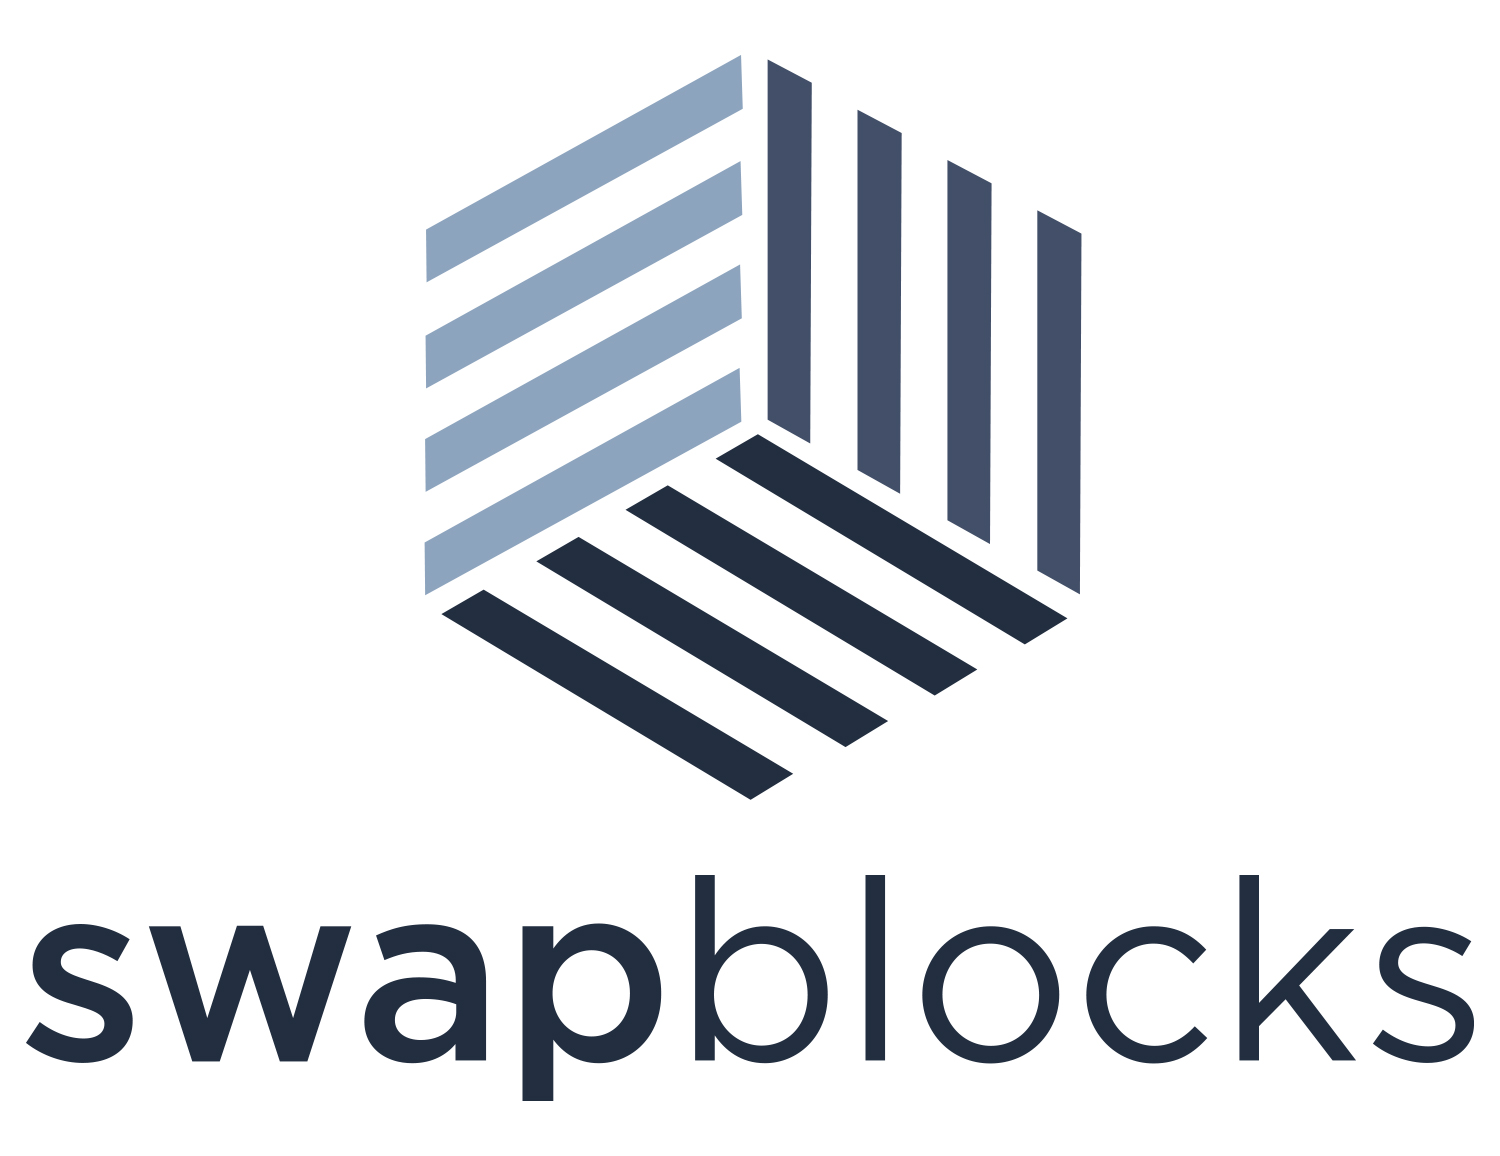
\includegraphics[width=6cm,height=5cm]{swapblocks_logo}
\\[\bigskipamount]
}



\title{Technical Specifications }
%\title{SWAPBlocks\\}
%\title{SWAPBlocks \\A Cost Saving Blockchain Protocol\\
%For Asset Issuance \& Exchange}
%\posttitle{A Cost Saving Blockchain Protocol\\
%For Asset Issuance \& Exchange}

	  
\author{Lance Rogers}

\date{\today}

\begin{document}

\maketitle


\section{SWAPBlocks Protocol}
\subsection{Base Protocol}
Assets are registered on the network by creating a new asset object containing 
a unique\_id, a pointer to the issuer, an asset\_id created by hashing the pointer 
and unique\_id, a prepended weight associated with the number of signatures needed 
for transactions to be considered valid and a valid\_through\_date.  Once the asset 
is created it is signed by the issuer and broadcast to the network as an asset 
genesis transaction. The issuer then runs a node supporting the network and listening 
for transactions containing its managed assets.

When a transaction is detected containing a managed asset the issuer processes the 
transaction and decides to approve or reject it.  This approval can be 
determined by any preset or future case set by the issuer.  Some examples include 
verifying that the address receiving the asset is legally allowed to receive the asset, 
verifying that an appropriate transaction fee has been included in the transaction, 
verifying that an encrypted form sent with the transaction contains the correct 
information, etc….  It is the responsibility of the issuer to provide counterparties with 
asset transfer instructions and the responsibility of the consumer to interpret
the instructions.

To approve a transaction the issuer must sign the transaction and rebroadcast 
the transaction to the network. Once the transaction is signed by the issuer
the transaction will be eligible for the next block.  
If the issuer does not approve the transaction it will
time out and be cleared from all network nodes.

\subsection{Consortium Extension}

The base protocol forces all transactions pertaining to a specific asset through 
the issuer's node which can cause performance issues and creates a single point 
of failure.  To solve these problems, issuers can extend the base protocol by 
forming consortiums that operate under consortium agreements.  These consortium 
agreements keep track of member nodes, consortium governing rules and 
verification scripts.  By joining a consortium the issuer agrees to process 
transactions of member nodes in accordance to the agreement and/or store 
the additional data attached to member transactions.

\section{Consortium}

Leaving an entity to verify all transactions pertaining to its managed assets can create 
a centralized bottleneck.  To solve this problem a municipal node can join or create a consortium.  
Consortiums are groups of nodes that require the same transaction verification process.  
This can be the full transaction verification needed or a subset of the full transaction verification. 
Consortiums follow rules set out in a consortium agreement which includes a transaction 
verification script, consortium data packet storage and routing fees.

Consortiums create a semi-decentralized, semi-private transaction verification network that 
enables a central entity to benefit from the distributed properties of a decentralized network.  
Consortiums also reduce the amount of trust needed to interact with any particular central 
entity since the operating agreement can be read and verified on the blockchain.

Consortiums use a group signature scheme which allows any member node to publicly verify a transaction on
behalf of the consortium
without publicly
exposing their identity.  However the consortium manager is able to identify the signer
of a message, allowing rogue group members to be exposed and kicked out of the consortium.



\begin{figure}[h]
	\centering
	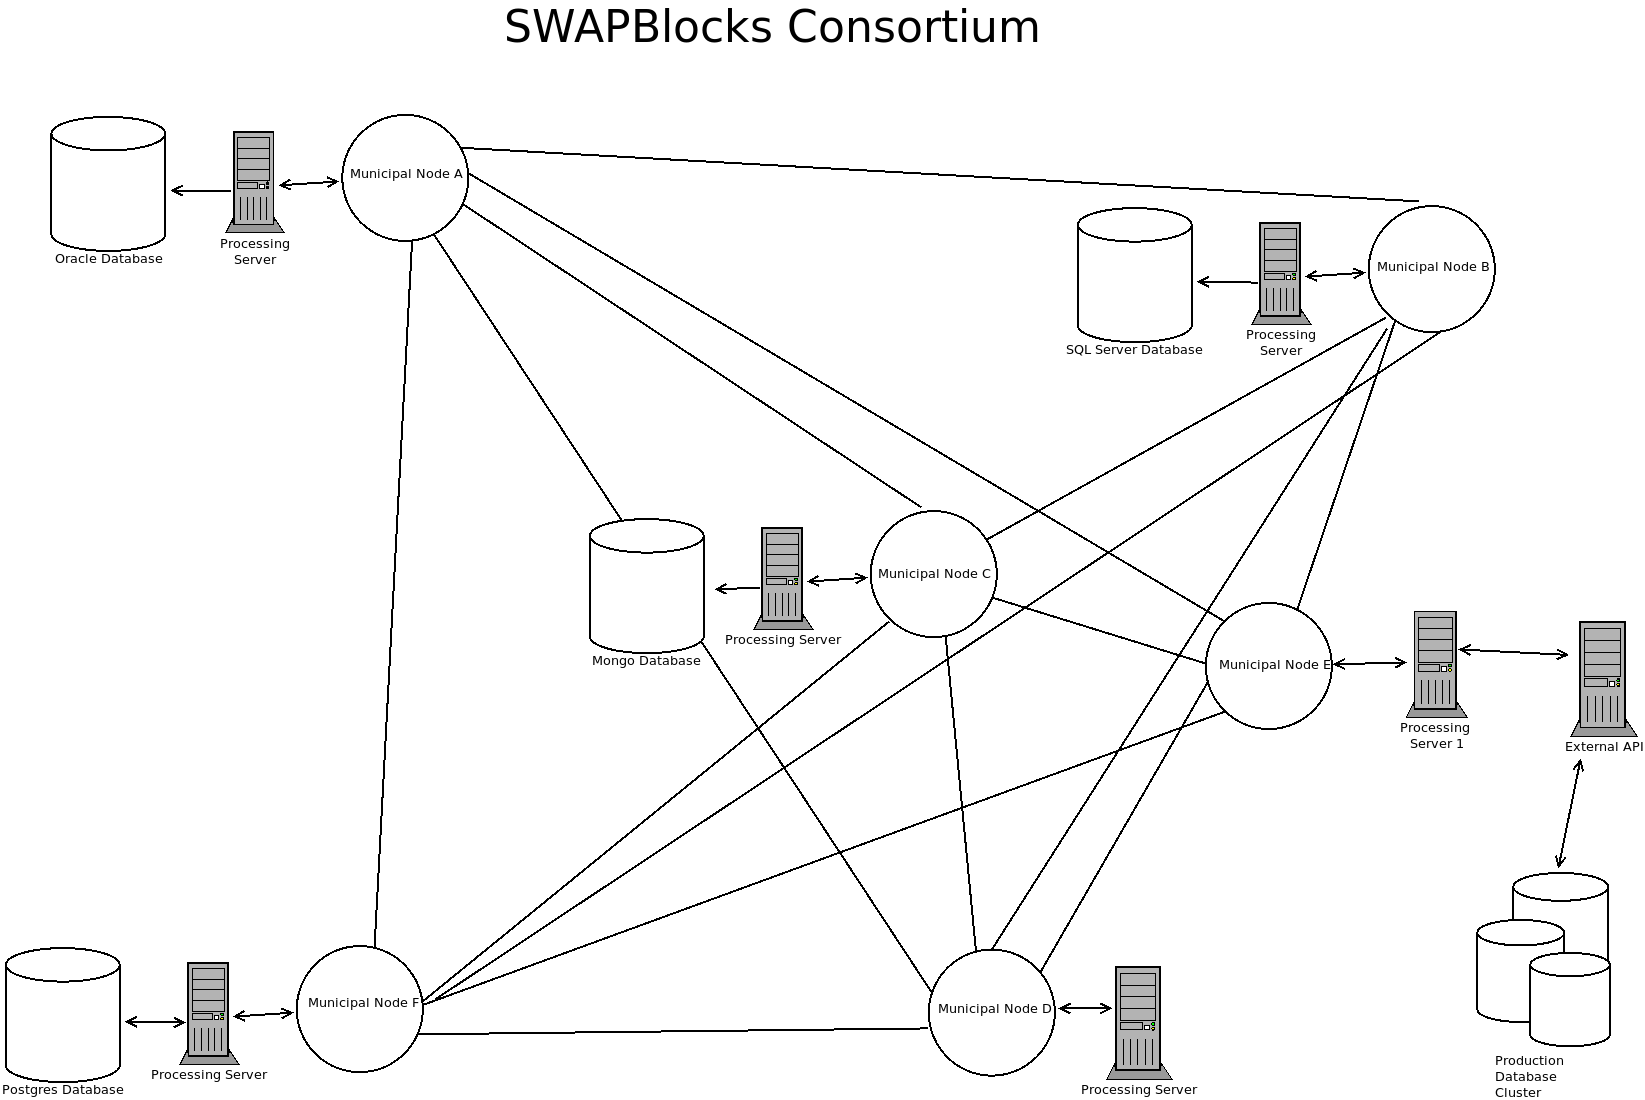
\includegraphics[width=.85\textwidth]{consortium}
	\caption{Consortium data storage infrastructure can vary between consortium nodes.} 
	\label{fig:consortium}
\end{figure}


\subsection{Consortium Agreement}

A consortium agreement is stored 
on the blockchain and acts as the operating agreement for all member nodes. 
This agreement outlines the processing script, consortium 
members, number of member signature needed for amendments, routing fee prices, a 
list of all member nodes' static IP’s, etc….

\subsection{Consortium Routing}


In order to limit the impact asset transactions have on the network as a whole mining 
nodes receive a portion of the attached fee for sending asset transactions to the correct
consortium network.  Consortiums can adjust the fee regularly to stay competitive for both
consumers and miners or build out a network. 
For a miner to 
increase their chances of receiving a routing fee they can store a dictionary 
of consortiums' node addresses for quick routing.



\subsection{Routing DAG}


The routing DAG contains the information associated with the routing of asset 
transfer transactions.  For example node X receives the transaction and performs standard 
verification, signs the transaction and broadcast it to the network where it is picked
by node Y. Node Y looks up the consortium's address in its dictionary of 
consortiums, signs and sends the transaction to consortium member node A. Node A performs 
consortium verification, signs the transaction and routes the transaction directly to 
municipal node F.  Node F verifies and signs the transaction. 
Now this transaction can be included in a block.  When the 
transaction is included in a block the last 3 addresses to sign the transaction 
receive shares of the attached routing fee.  Each signature in the routing DAG points 
to the previous one and can only contain one signature per level of verification.  
The first signature can be any node in the network, 
the second signature can be either a consortium member or the municipal node 
and the third can only be the municipal node.  The amount of signatures needed 
is determined by the asset's assigned weight value. 
%There will be a disincentive for altering the DAG.




\section{Node States}

SWAPBlocks assets view nodes in three different states. The state that the node is viewed in 
by the asset determines the level of verification the node is allowed to and should
perform.


\begin{enumerate}
	\item Standard Node State
		\begin{itemize}
			\item{Any network node that has no ownership stake in an asset}
			\item{Checks that each transaction output points to valid UTXOs
				and that all signatures are correct.}
		\end{itemize}
	\item Consortium Node State
		\begin{itemize}
			\item{Node belongs to the same consortium as the asset issuer,
				thus abiding by the same consortium agreement.}
			\item{Typically responsible with processing  or storing
				consortium data packets containing information 
				needed for additional verification}
		\end{itemize}
	\item Municipal Node State
		\begin{itemize}
			\item{Node owned by the asset issuer.}
			\item{Responsible for verifying municipal data packets.}
			\item{Responsible with updating their own outside record keeping systems 
				with status changes of registered assets.}	
		\end{itemize}
\end{enumerate}

\begin{figure}[h]
	\centering
	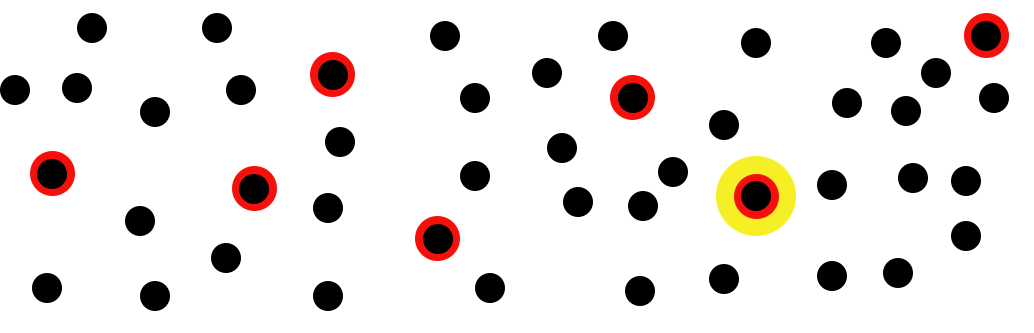
\includegraphics[width=.85\textwidth]{node_space}
	\caption{Node space in relation to some registered asset}
	\label{fig:nodespace1}
\end{figure}


Figure \ref{fig:nodespace1} represents the node space in relation to a registered asset.
Each circle represents a node and each color represents the state that the
node is in for a particular asset.  The yellow circle represents the municipal node, meaning
that the yellow node registered and manages the asset.  The red circles represent consortium 
nodes, meaning that each red node is a member of the same consortium as the municipal node.
The black dots represent standard network nodes that do not have any special permission or
obligation to provide additional verification for this asset.

%As you can see each node state inherits the traits of the previous state.





\section{Asset Registration}

Municipal nodes register assets in an asset genesis transaction.  When 
an asset is registered there are only 4 required fields, the registering node's 
pub key, the consortium's address if there is one, a UAI and a valid\_through date.  
This valid\_through date is the date that the entity guarantees the information 
about the asset to be correct.  The asset must be verified through an asset probe 
transaction to update the valid\_through date.

\subsection{Asset ID}

Assets on the SWAPBlocks network are represented by a unique asset ID (UAI).  
The UAI is created by hashing the consortium address with the municipal address 
and then hashing that with the municipal ID to create the base\_id.


% ASSET ID DIAGRAM HERE


% Add below to diagram somehow
% Asset Base ID:
% e3cc54301269c1c54afeb86e4391a9ad80d40484a9b0db0e6618b835decc9628

Now that the base ID has been formed the municipal node assigns 
a weight, determining the level of verification required to transfer 
the asset, and prepends the weight to the beginning of the asset ID.

\subsection{Weights}

Assets are assigned weights when they are first created. These weights are used to
to determine the level of verification a transaction containing the asset needs before
being eligible to be
included in the next block. Weight is calculated based on the number of valid signatures
a transaction has in it's routing DAG.


\begin{itemize}
	\item Weight 0, Standard Verification
		\begin{itemize}
			\item{Default verification requiring the transaction to include
				valid UTXOs and signatures.}
		\end{itemize}
	\item Weight 1, Consortium Level Verification
		\begin{itemize}
			\item{Transactions must pass weight 1 verification and contain an
				additional signature from a consortium node.}
			\item{Assets with this weight may require a consortium data packet
				to be sent along with every transfer transaction}
		\end{itemize}
	\item Weight 2
		\begin{itemize}
			\item{Transactions must pass weight 0 verification and include a 
				municipal signature in the routing DAG.}
			\item{Consortium nodes can perform consortium verification on
				the consortium data packet, sign the DAG and send the
				transaction directly to the municipal node, enabling
				the consortium node to receive some of the routing fee.
				If this verification has been done and signed off by
				a trusted consortium node the municipal node does not
				need to reverify and will only need to
				perform municipal verification.}
		\end{itemize}
\end{itemize}

% ADD Weighted Asset Diagrams Here


\section{Transactions}

\subsection{Transaction Types}
There are 5 basic types of transactions in the SWAPBlocks ecosystem.

\begin{enumerate}
	\item Currency
		\begin{itemize}
			\item{Involves the transfer of SBX coins from one address to another.}
			\item{Currency transactions can be validated by checking UTXOs and the
				validation can be performed by every node in the network.}
		\end{itemize}
	\item Asset Genesis
		\begin{itemize}
			\item{Transaction that registers an asset on the network for the first time.}
		\end{itemize}
	\item Asset Transfer
		\begin{itemize}
			\item{Transaction used to send an asset from one account to another
				with no contingencies.}
		\end{itemize}
	\item Asset Swap
		\begin{itemize}
				
			\item{Transaction in which two parties agree to swap 
				ownership of two assets with the contingency that 
				each transaction clears before the swap completes.}
			\item{Contains maker and taker sections. Both sections must
				be complete and verified for the transaction to be eligible for
				the next block.}
			\item{Consist of two transaction types, LOCK and UNLOCK.} 
				\begin{itemize}
					\item{LOCK transactions lock the asset swaps in the opposing wallets.}  
					\item{Requires an UNLOCK transaction be broadcast to finalize ownership of the new assets. If an UNLOCK transaction is not broadcast before the valid\_to\_date, the swap transaction reverses.}
				\end{itemize}
			\item{If the bid section is blank, then the transaction will be considered pending and can
				be filled by any bidder and rebroadcast to the network. These pending SWAP transactions
				will be stored in the SWAP order book, which is like a mempool for SWAP transactions.} 
		\end{itemize}
	\item Asset Probe
		\begin{itemize}
			\item{Transaction completed by the asset issuer or 
				trusted third party that validates that the asset's condition 
				is the same as the current record stored by the issuer.}
			\item{These will have to be 
				completed periodically to ensure the asset has not been 
				discarded, destroyed or transferred off network.}
			\item{Managing 
				entities can charge fees to complete an asset probe transaction 
				for an asset they manage.}
			\item{Asset probe transactions can also 
				be completed by third party networks and will be linked to 
				the assets transaction chain but the valid\_through date 
				will still remain the same.}
		\end{itemize}
\end{enumerate}

% TRANSACTION DIAGRAMS HERE

\subsection{SWAP Order Book (The SWAP DEX)}
The SWAP order book is a specialized mempool for storing unverified SWAP transactions.  What this means is that
all SWAP transactions without a counterparty will be stored in a separate mempool for quick lookup. 
Decentralized exchange portals will be able to utilize this mempool to quickly place and fulfil orders.


\subsection{Transaction Timeout}


In order to limit the number of unverified transactions in the mempool, 
transactions are created with a max\_verify\_time.  The max\_verify\_time
is the latest time a transaction may be kept in the mempool.  If a node has 
transactions in its mempool past the max\_verify\_time the node can discard 
the transactions.  This helps to prevent spam transactions from bloating the 
mempool without needing to charge a fee.

For verified transactions 
that have not been included in a block and that contain data packets, the max\_verify\_time
acts as a data\_storage time limit.  Once the max\_verify\_time has been reached all nodes 
can delete the data packets of non-consort assets, leaving only the hash value.

The max\_verify\_time will have a constant max time on network launch.  
In the future a proof of importance algorithm may be used to 
allow users to extend the max\_verify\_time.

To prevent users from issuing transactions with an extremely long max\_verify\_time, a 
transaction's max\_verify\_time
must be less than or equal to a network constant as part of standard verification.

\section{Permissioned Smart Contracts}

SWAPBlocks enables asset transactions to include temporary encrypted data packets. These data
packets are used by municipal and consortium nodes to make verification decisions.  Asset transactions
can include two separately encrypted data packets for multi-level verification and increased privacy.

\begin{enumerate}
	\item Consortium Data Packet:
		\begin{itemize}
			\item{Contains information that can be verified by consortium member
				nodes.}
			\item{Enables entities to validate standard form data quickly.} 
			\item{This data packet is typically spread across the consortium for backup
				and high availability.}
			\item{Data is encrypted with a randomly generated key that is then encrypted
				with the consortium's public key and added to the transaction.}
			\item{All consortium members have access to a shared key pair}	
		\end{itemize}
	\item Municipal Data Packet:
		\begin{itemize}
			\item{Contains information that is either confidential or that the
				consortium has not agreed to process.}
			\item{Can only be verified by municipal nodes}
			\item{Only stored by municipal nodes}
		\end{itemize}
\end{enumerate}

Once the data packet has been verified by the approved node, the node signs the 
transaction. This signature is added to the routing DAG and the transaction is either routed
		to the next required level or broadcast to the network.
When a transaction's DAG has reached 
its required weight, the transaction can be included in the next block and the data
		packet will be cleared from all non-member nodes.

If the data packet has not passed verification the verifying node will not sign the transaction
leaving the transaction to time out and be cleared from all network nodes.

This verification process can be thought of as using permissioned smart contracts.  In the case of municipal
verification, registering accounts are the only approved account to run the verification script on the asset.
With consortium verification the smart contract will be defined in the consortium agreement.


\section{Decided/Undecided Protocol Specifications}
\begin{enumerate}
	\item{Consortium and municipal packets will be encrypted with AES-256 by default.}
	\item{All hashes should use SHA-3 256 (Keccak)}
	\item{Default compression and encryption of data packets not yet decided}
		\begin{enumerate}
			\item{Will need to take into consideration compression duplication of common values}
			\item{Need to consider size of data packet and padding}
			\item{Need to consider time to send data transmission}
			\item{Need to consider chaining transactions to send large packets}
		\end{enumerate}
	\item{Consortiums will be based on a 
			\href{https://dl.acm.org/citation.cfm?id=1754897}{Group Signature Scheme as first described by Chaum and Van Heyst}
		}
		\begin{enumerate}
			\item{Particular scheme not yet decided}
			\item{Possibilities:}
				\begin{enumerate}
					\item{\href{https://eprint.iacr.org/2008/047.pdf}{“Fair traceable multi-group signatures”}}
					\item{\href{https://eprint.iacr.org/2008/112.pdf}{“Democratic Group Signatures with Threshold Traceability” by Zheng et al.}}
					\item{\href{https://pdfs.semanticscholar.org/dfd3/0ee27ab7167900dbdddff11b22132f9ea5d5.pdf}{“Short group Signatures with Distributed Traceability” by Blomer et al.}}
				\end{enumerate}
		\end{enumerate}
\end{enumerate}



\end{document}
